\chapter{Performance Bottlenecks in \CZTS}

\section{Thermodynamic Disordering of Cu \& Zn Ions in \CZTS}
\subsection{Spatial Extent of Disorder Amongst Cu and Zn Cations}
\begin{itemize}
\item Recovery of kesterite ground state at T=50k? (Cu-Zn and Cu-Sn layers, see lab book pg 2): visuals of structure in VESTA and RDF of Cu-Zn and Cu-Sn pairs
\item Visuals of configs from eris and RDFs across T range 
\end{itemize}
\subsection{Band Tailing due to Fluctuations in Electrostatic Potential}
R plots for distributions of electrostatic potential of Sn

\section{Formation Energy of Sulfur Vacancies}
We investigate the formation energy of charge neutral sulfur vacancies (V$_{S}^{0}$) as a function of the sulfur chemical potential, which itself is a function of temperature and pressure. We therefore can assess the formation energy of the vacancy under typical annealing conditions. Work from Scragg et al showed that annealing out Cu and Zn disorder can be a very time consuming process, therefore for most practical purposes some disorder will be `frozen in' after annealing. Typical annealing conditions for { \CZTS } are at ?? K and it has been shown that lower pressures are more optimal for the sulfide (whereas higher pressures are better for the selenide) **cite Adam?**. This is due to the allotropes of S?\\

On -going calculations are being performed for the charged sulfur vacancies (V$_{S}^{+1}$ and V$_{S}^{+2}$) so that the minimum energy defect, accounting for all possible charge states, across the temperature and pressure range can be determined.

\begin{figure}[h!]
  \centering
    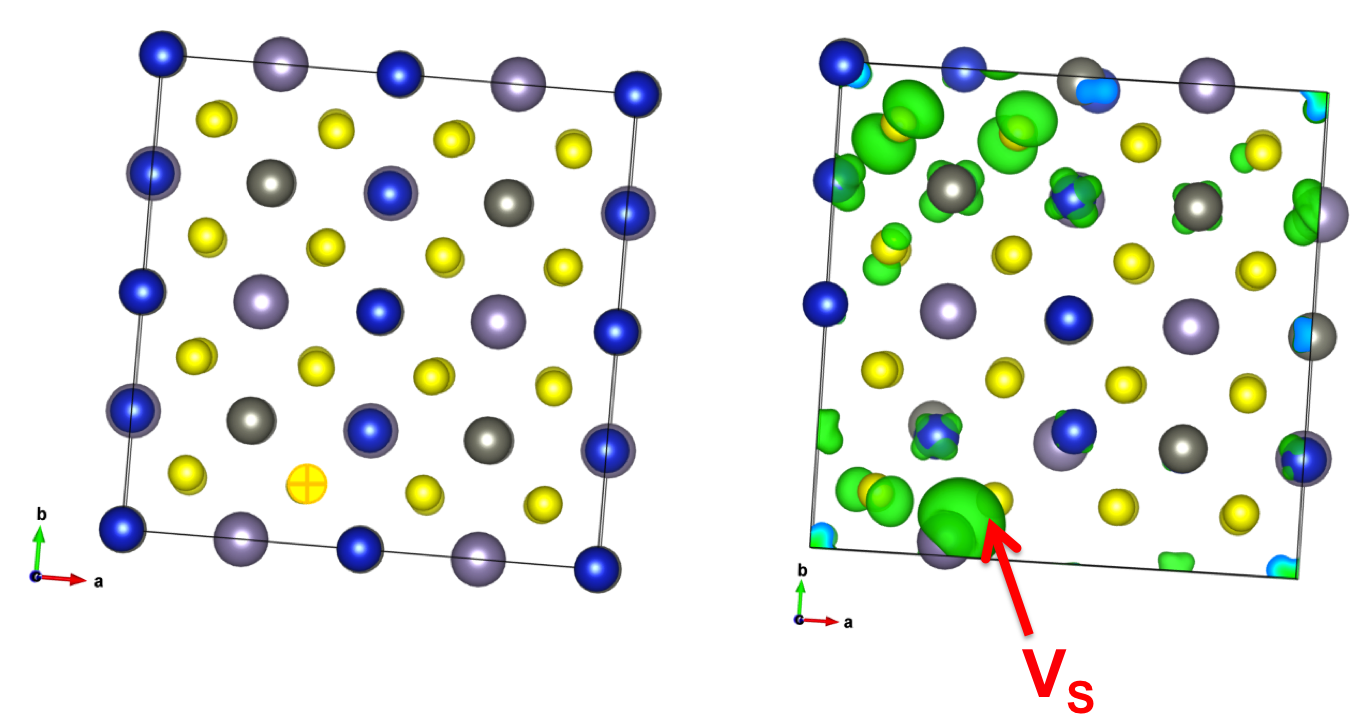
\includegraphics[width=0.9\textwidth]{figures/V_S-neutral-PARCHG.png}
    \caption{Perfect {\CZTS } supercell with S anion removed to form a sulfur vacancy (V$_S$) indicated by a crosshair (left) and the calculated partial charge density of two excess electrons present for the charge neutral V$_S$ (right).}
  \label{V_S-neutral-PARCHG}
\end{figure}

\section{Intrinsic Band Gap Broadening from Lattice Vibrations}
For CZTS we find that the band gap decreases with temperature as a result of lattice dilation, which a trend observed in most typical semiconductors such as Si, Ge and GaAs. *see slide show results* -- discuss deformation potential, elastic constant and band gap broadening as a function of T (fundamental intrinsic limit to charge-carrier mobilities) + discuss than we calculate just one contribution to the broadening currently to compare to expt to determine how much is intrinsic and how much is defect-related. Although we calculate only gamm-acoustic as opposed to LO? see MAPI paper eqn1

`typical semiconductors such as Si, Ge and GaAs, for which the bandgap decreases with temperature as a result of lattice dilation26,37' \cite{MAPI_Eg_broadening} 

`electron–phonon coupling at room temperature is almost solely governed by deformation potential scattering with acoustic phonons, which is known18,25 to theoretically result in mpT?3/2' \cite{MAPI_Eg_broadening}

